%!TEX root = ../thesis.tex
\chapter{User studies and Results}
\label{chap:results}

The results of this study were determined by the answers to a survey completed by the users that participated in the testing phase. \\
\noindent We recruited 6 people from Uppsala University and asked them to use the application for a period of 2 weeks and fill up a survey with 26 questions (see Appendix). The survey is anonymous and divided in 3 sections: the first part was designed to gather the information related to the audience. The second part aimed to rate the interest in learning a new language using a mobile device, and the third part was dedicated to the application itself. \\

\section{Audience}
\label{sub:Audience}

This section presents the answers related to the users personal information to get a better understanding of the audience. From Figures~\ref{fig:gender_chart} and \ref{fig:age_chart} we can say that the majority of our users are male and between the age of 24-29 years old.  Table \ref{table:native_languages} describes the native language of the users.

\begin{figure}[!ht]
	\centering
	\begin{minipage}{.5\textwidth}
		\centering
		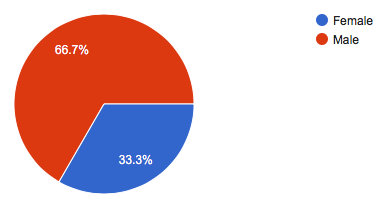
\includegraphics[scale=0.5]{Figures/responses/audience_gender.png}
		\caption{Gender chart}
		\label{fig:gender_chart}
	\end{minipage}%
	\begin{minipage}{.5\textwidth}
		\centering
		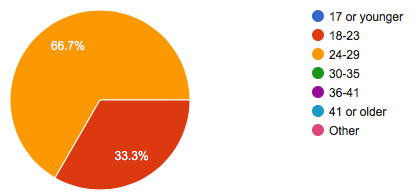
\includegraphics[scale=0.5]{Figures/responses/audience_age.png}
		\caption{Age chart}
		\label{fig:age_chart}
	\end{minipage}
\end{figure}

\begin{table}[!ht]
    \centering
    \begin{tabular}{|l|c|}
        \hline
        \multicolumn{1}{|c|}{\textbf{Native language}} & \textbf{Amount} \\ \hline
        Italian                                        & 2               \\ \hline
        Greek                                          & 2               \\ \hline
        Swedish                                        & 1               \\ \hline
        Arabic                                         & 1               \\ \hline
    \end{tabular}
    \caption{Users native languages}
    \label{table:native_languages}
\end{table}

\noindent All testers were students from the Computer Science department as well as comfortable in using mobile applications on a daily basis.

\section{Interest}
\label{sub:Interest}

This section describes the interest of our testers in learning and improving a new language using a mobile application instead of the traditional student-teacher class. Results are very positive and confirm that the interest is high. In particular, avoiding the interaction with a physical teacher is very welcomed. In fact, the interest in not having this sort of supervision, the \textit{standard deviation} is $0.8367$, the \textit{mean} is $4.5$ and the \textit{variance} is $0.7$ (Figure~\ref{fig:int_no_teacher}).

\begin{figure}[!ht]
	\centering
	\begin{minipage}{.5\textwidth}
		\centering
		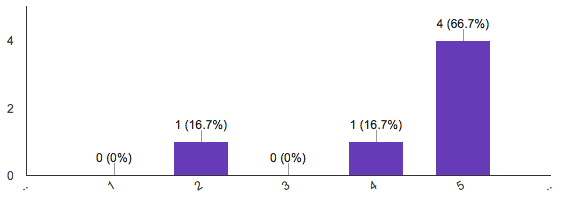
\includegraphics[scale=0.4]{Figures/responses/interest_learning_language.png}
		\caption{Interest in learning a new language}
		\label{fig:int_learnign_lang}
	\end{minipage}%
	\begin{minipage}{.5\textwidth}
		\centering
		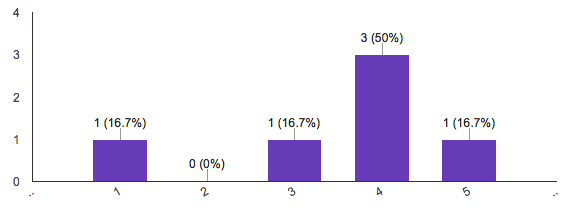
\includegraphics[scale=0.4]{Figures/responses/interest_improving_lang.png}
		\caption{Interest in improving English language}
		\label{fig:int_improving_lang}
	\end{minipage}
    \begin{minipage}{.5\textwidth}
        \centering
        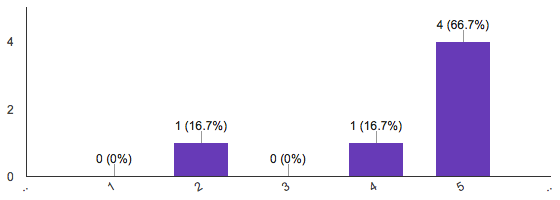
\includegraphics[scale=0.4]{Figures/responses/interest_usage_smartphone.png}
        \caption{Interest in using a smartphone}
        \label{fig:int_usage_smartphone}
    \end{minipage}%
	\begin{minipage}{.5\textwidth}
		\centering
		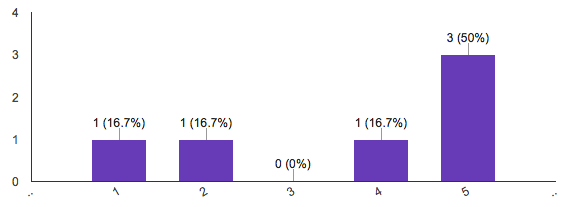
\includegraphics[scale=0.4]{Figures/responses/interest_visual_feedback.png}
		\caption{Interest in having visual feedback}
		\label{fig:int_visual_feedbak}
	\end{minipage}%
\end{figure}

\noindent Learning a new language has received a positive interest because the \textit{mean} is $4.3$ with a \textit{standard deviation} of $1.21106$ and a \textit{variance} of $1.4667$ (Figure~\ref{fig:int_learnign_lang}). This indicates that users are eager to acquire new linguistic competencies. The same positive interest was given to the usage of a smartphone as a way of learning. In fact the \textit{mean} is $4.3$ with a \textit{standard deviation} of $1.21106$ and a \textit{variance} of $1.4667$ (Figure~\ref{fig:int_usage_smartphone}). These two results go along with the fact that people want to learn new languages and avoid the direct supervision with a teacher. The usage of a smartphone is an effective way for delivering linguistic knowledge. \\

\noindent A slight difference was observed concerning the English pronunciation and the visual feedback. In fact, according to our results, people are more interest in acquiring new languages rather then improving the one that they have already a good knowledge of. Looking at the results, we observed that the interest of improving English has a \textit{mean} of $3.5$ with a \textit{standard deviation} of $1.3784$ with a \textit{variance} of $1.9$ (Figure~\ref{fig:int_improving_lang}), whereas, the interest of using visual feedback as approach of learning has a \textit{mean} of $3.667$ with a \textit{standard deviation} of $1.7512$ with a \textit{variance} of $3.0667$ (Figure~\ref{fig:int_visual_feedbak}).

\begin{figure}[!ht]
	\centering
	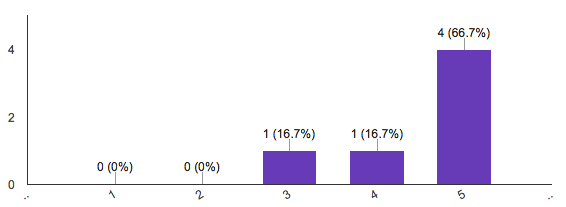
\includegraphics[scale=0.4]{Figures/responses/interest_no_teacher.png}
	\caption{Interest in not having a teacher's supervision}
	\label{fig:int_no_teacher}
\end{figure}

\section{Application}
\label{sub:Application}
\noindent The following charts are the results of the survey's questions related to the application itself. The questions were designed in order to understand the feelings about how the users understood the different features provided by the application. These questions are divided into three sub-categories: the first one is related to a broad view of the product, the second category aims to define the \textit{understanding} of the users about the features, whereas the third one, how useful these features are in order to improve the pronunciation. \\

\noindent The \textit{general appreciation} received a positive feedback. In fact, the \textit{mean} is $3.33$ with a \textit{standard deviation} of $0.8165$ and a \textit{variance} of $0.667$ (Figure~\ref{fig:application_liked}). Also, the users have expressed a positive interest in continuing using the application if there would be a real product on the market in the future. The \textit{mean} is $3.1$ with a \textit{standard deviation} of $0.753$ and a \textit{variance} of $0.5667$ (Figure~\ref{fig:understanding_main} ). As last question of this first sub-category, we asked \textit{"how difficult was the usage"} of the entire system. Users responded with a \textit{mean} of $4$ with a \textit{standard deviation} of $1.0954$ and a \textit{variance} of $1.2$ (Figure~\ref{fig:application_usage}).

\begin{figure}[!ht]
	\centering
	\begin{minipage}{.5\textwidth}
		\centering
		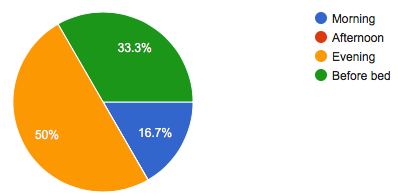
\includegraphics[scale=0.4]{Figures/responses/application_period_of_usage.png}
		\caption{Moment of the day}
		\label{fig:application_period_of_usage}
	\end{minipage}%
	\begin{minipage}{.5\textwidth}
		\centering
		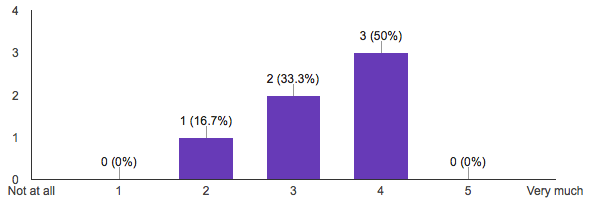
\includegraphics[scale=0.4]{Figures/responses/application_liked.png}
		\caption{General appreciation}
		\label{fig:application_liked}
	\end{minipage}%
\end{figure}

\begin{figure}[!ht]
	\centering
	\begin{minipage}{.5\textwidth}
		\centering
		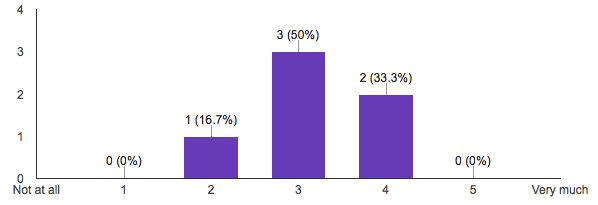
\includegraphics[scale=0.4]{Figures/responses/application_usage.png}
		\caption{Interest in continuing using the application}
		\label{fig:application_usage}
	\end{minipage}%
	\begin{minipage}{.5\textwidth}
		\centering
		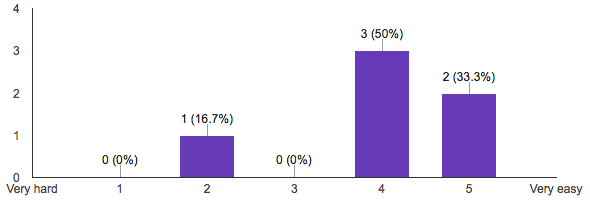
\includegraphics[scale=0.4]{Figures/responses/application_usage_difficulty.png}
		\caption{Usage difficulty}
		\label{fig:application_usage_difficulty}
	\end{minipage}
\end{figure}

\noindent The \textit{"Understanding"} sub-category received a slightly different appreciation level. In fact, according to the results of the survey, the users had some difficulties in understanding the usage of the charts in the feedback page. However, regarding the main page and the critical listening, the results were still positive. The main page received a \textit{mean} value of $3.833$ with a \textit{standard deviation} of $1.1691$ and a \textit{variance} of $1.3667$ (Figure~\ref{fig:understanding_main}), whereas the critical listening had a \textit{mean} of $4.167$ with a \textit{standard deviation} of $0.9832$ and a \textit{variance} of $0.9667$ (Figure~\ref{fig:understanding_listening}). Basically, the users clearly understood the meaning and the usage of all the functionalities regarding the two pages in the application. \\
\noindent The main overview of the feedback page did receive good feedback as well. In fact we had a \textit{mean} of $3.1667$ with a \textit{standard deviation} of $1.1691$ and \textit{variance} of $1.3668$ (Figure~\ref{fig:understanding_feedback}). Despite these results, the inner functionalities of the feedback page, have received low scores. According to the results, the \textit{vowels charts} had the lowest \textit{mean}, with a value of $2.5$ and a \textit{standard deviation} of $0.837$ and \textit{variance} of $0.7$ (Figure~\ref{fig:understanding_vowels}). This a clear indication that the users did not properly understood the way the chart worked. The \textit{pitch trend chart} received a slightly better score with a \textit{mean} of $2.667$ and a \textit{standard deviation} of $1.0328$ with a \textit{variance} of $1.0667$ (Figure~\ref{fig:understanding_pitch}). \\
\noindent The \textit{stress} had a \textit{mean} of $2.667$ with a \textit{standard deviation} of $0.8165$ and \textit{variance} of $0.667$ (Figure~\ref{fig:understanding_stress}), whereas the \textit{history page} had a \textit{mean} of $3.5$ with a \textit{standard deviation} of $1.0489$ and \textit{variance} of $1.1$ (Figure~\ref{fig:understanding_history}).

\begin{figure}[!ht]
	\centering
	\begin{minipage}{.5\textwidth}
		\centering
		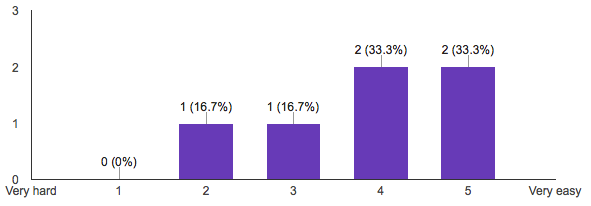
\includegraphics[scale=0.4]{Figures/responses/understanding_main.png}
		\caption{Understanding the main page}
		\label{fig:understanding_main}
	\end{minipage}%
	\begin{minipage}{.5\textwidth}
		\centering
		\includegraphics[scale=0.4]{Figures/responses/understanding_listening.png}
		\caption{Understanding the critical listening page}
		\label{fig:understanding_listening}
	\end{minipage}
	\begin{minipage}{.5\textwidth}
		\centering
		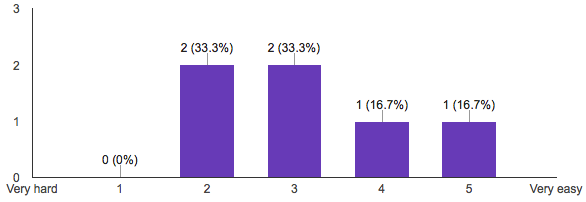
\includegraphics[scale=0.4]{Figures/responses/understanding_feedback.png}
		\caption{Understanding feedback page}
		\label{fig:understanding_feedback}
	\end{minipage}%
\end{figure}

\begin{figure}[!ht]
	\centering
	\begin{minipage}{.5\textwidth}
		\centering
		\includegraphics[scale=0.4]{Figures/responses/understanding_stress.png}
		\caption{Understanding stress on a sentence}
		\label{fig:understanding_stress}
	\end{minipage}%
	\begin{minipage}{.5\textwidth}
		\centering
		\includegraphics[scale=0.4]{Figures/responses/understanding_pitch.png}
		\caption{Understanding pitch trend}
		\label{fig:understanding_pitch}
	\end{minipage}
	\begin{minipage}{.5\textwidth}
		\centering
		\includegraphics[scale=0.4]{Figures/responses/understanding_vowels.png}
		\caption{Understanding vowels chart}
		\label{fig:understanding_vowels}
	\end{minipage}%
	\begin{minipage}{.5\textwidth}
		\centering
		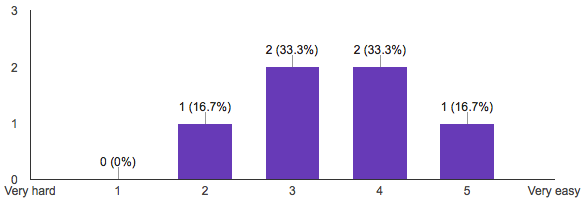
\includegraphics[scale=0.4]{Figures/responses/understanding_history.png}
		\caption{Understanding history page}
		\label{fig:understanding_history}
	\end{minipage}%
\end{figure}

\noindent The last sub-category is regarding on \textit{"how useful are the features"} in order to improve the pronunciation. Unfortunately, the users did not find the \textit{listening} or the \textit{history} to be useful. In fact, for the first one, we had a \textit{mean} of $2.167$ with a \textit{standard deviation} of $1.329$ and a \textit{variance} of $1.767$ (Figure~\ref{fig:utility_listening}), and the second one had a \textit{mean} of $1.667$ with a \textit{standard deviation} of $0.816$ and \textit{variance} of $0.667$ (Figure~\ref{fig:utility_history}). These results clearly show that the feeling of the users regarding these two functionalities were very similar. Slightly better for the feedback page: we had a \textit{mean} of $2.33$ with a \textit{standard deviation} of $1.211$ and a \textit{variance} of $1.467$ (Figure~\ref{fig:application_rate_feedback}). \\
\noindent The very last question aimed to find out whether the users actually improved the pronunciation or not. The results were not particularly encouraging because we had a \textit{mean} of $2.167$ with a \textit{standard deviation} of $1.329$ and a \textit{variance} of $1.767$ (Figure~\ref{fig:application_improved_pronunciation}).

\begin{figure}[!ht]
	\centering
	\begin{minipage}{.5\textwidth}
		\centering
		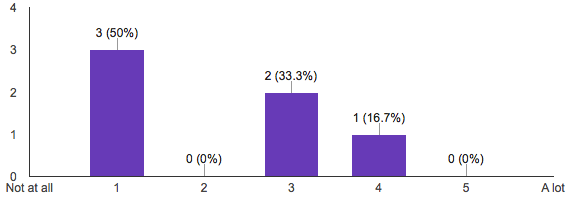
\includegraphics[scale=0.4]{Figures/responses/application_improved_pronunciation.png}
		\caption{Pronunciation improved}
		\label{fig:application_improved_pronunciation}
	\end{minipage}%
	\begin{minipage}{.5\textwidth}
		\centering
		\includegraphics[scale=0.4]{Figures/responses/utility_of_listening.png}
		\caption{Utility of critical/self listening}
		\label{fig:utility_listening}
	\end{minipage}
	\begin{minipage}{.5\textwidth}
		\centering
		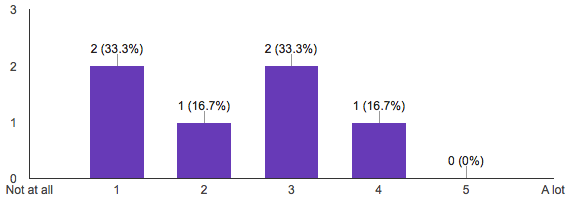
\includegraphics[scale=0.4]{Figures/responses/application_rate_feedback.png}
		\caption{Utility of feedback}
		\label{fig:application_rate_feedback}
	\end{minipage}%
	\begin{minipage}{.5\textwidth}
		\centering
		\includegraphics[scale=0.4]{Figures/responses/utility_of_history.png}
		\caption{Utility of history page}
		\label{fig:utility_history}
	\end{minipage}%
\end{figure}
